
%---------------Generación de señales------------------
\subsection{Generación de señales}

Se considera la función senoidal $s(t) = Asin(2\pi ~f~t + \phi)$, donde A es la amplitud de la señal, $t$ es el tiempo en segundos, $f$ es la frecuencia en Hz y $\phi$ la fase de la señal en radianes. Se buscará generar la función de tiempo discreto $s[n] = Asin(2\pi (f/f_s)n + \phi)$, donde $f_s$ es la frecuencia de muestreo en \textit{sps},  y $n~\in \left\lbrace \mathbb{N} + 0 \right\rbrace\ $

\begin{enumerate}
    \item Se generan dos señales sinusoidales de frecuencias $50~Hz$ y $500~Hz$, con duración de $1~seg$, la misma fase inicial y amplitud unitaria.
    
    Se escoge una frecuencia de muestreo $f_s = 4~kHz$, dado que este valor cumple holgadamente el criterio de Nyquist según el teorema del Muestreo, además cumple también este criterio para trabajar las frecuencias presentes en actividades posteriores.
    
    La figura \ref{s50_s500} muestra las gráficas obtenidas usando el comando \texttt{plot} a las señales  de frecuencias $50~Hz$ y $500~Hz$, antes mencionadas.
    
    \begin{figure}[H]
        \centering
        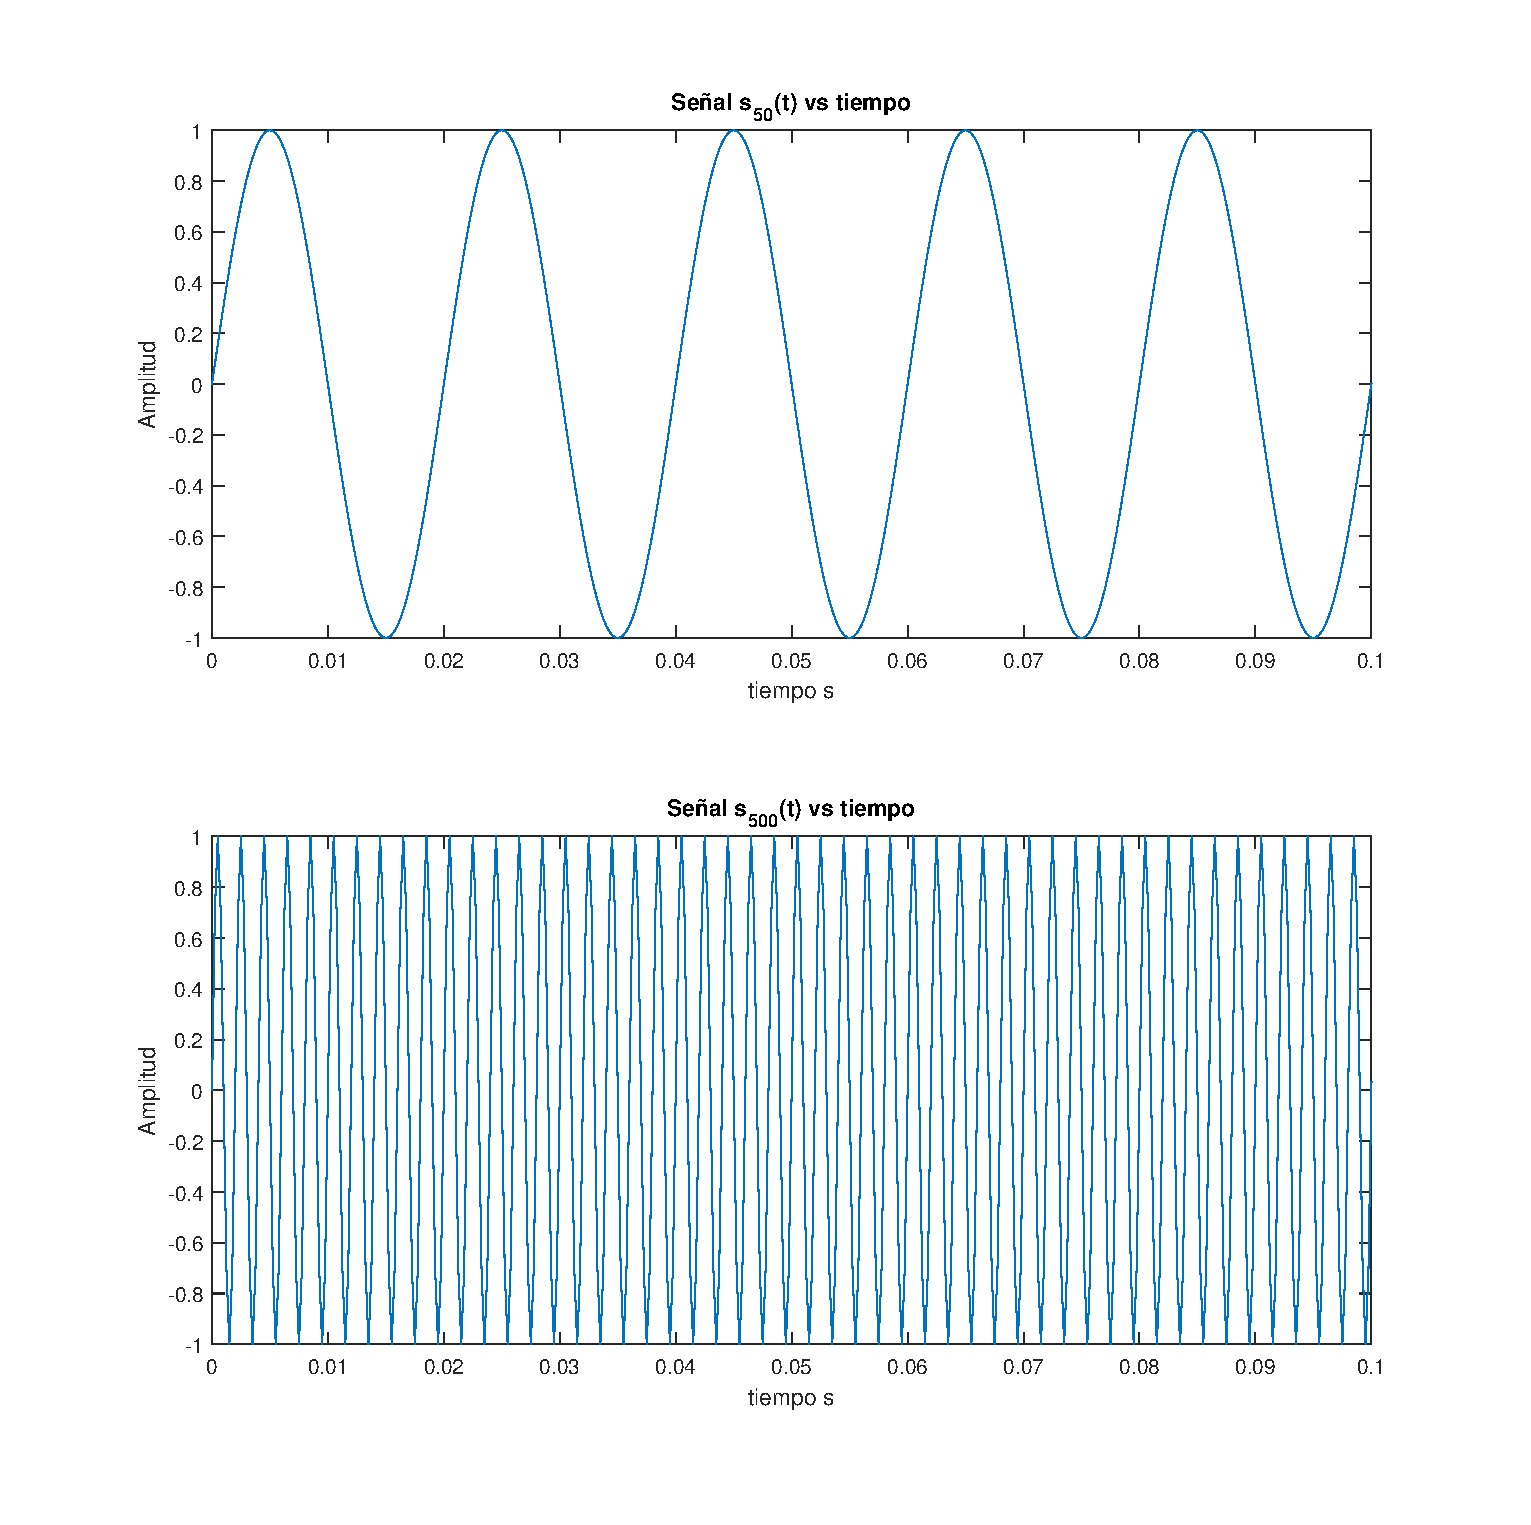
\includegraphics[scale = 0.6]{Imagenes/s50_s500.eps}
        \caption{Gráfica de las señales sinusoidales de  de frecuencias $50~Hz$ y $500~Hz$ generadas.}
        \label{s50_s500}
    \end{figure}
    
    Al reproducir estas señales con el comando \texttt{soundsc}, se puede notar que la señal de frecuencia $50~Hz$  es apenas audible, mientras que la que tiene una frecuencia de $500~Hz$  se logra percibir claramente como un tono puro.
    
    
    \item   Al hacer la suma las dos señales generadas de frecuencias $50~Hz$ y $500~Hz$, se obtiene una señal de $500~Hz$ montada sobre una señal de $50~Hz$, es decir, esta señal resultante conserva el periodo de su componente de menor frecuencia, en este caso $0.02~s$ Esto se puede ver en la primera gráfica de la figura \ref{suma_senos}
    
    
    Al realizar esta misma prueba de sumar dos señales sinusoidales, pero esta vez siendo de frecuencias de $200~Hz$ y  $300~Hz$, Lo que se obtiene es una señal que mezcla ambas componentes,  pero con un periodo de $0.01~s$, como se ve en la segunda gráfica de la figura \ref{suma_senos} Se empieza a notar el comportamiento de una señal generada por la suma de dos sinusoides, donde la frecuencia fundamental de esta señal resultante corresponde al máximo común divisor entre las frecuencias de las componentes de la señal, siendo en este caso de $100~Hz$
    
    Finalmente al componer el acorde de \textit{LA}, sumando tres señales sinusoidales con frecuencias de $880~Hz$, $100~Hz$ y $1320~Hz$ se deduce que la señal resultante deberá tener como frecuencia fundamental el máximo común divisor entre las frecuencias que la componen, en este caso de $220~Hz$, por lo que se tiene que las  frecuencias utilizadas corresponden a los armónicos 4,5 y 6 respectivamente de la nota LA2.
    
    
    Al reproducir la primera señal generada, en donde una de sus componentes coincide con la frecuencia fundamental resultante lo que se escucha son dos tonos por separado, mientras que en los dos últimos casos, donde la frecuencia fundamental resultante no se encuentra entre las componentes que la formaron se escucha un sonido más homogéneo.
    
    \begin{figure}[H]
        \centering
        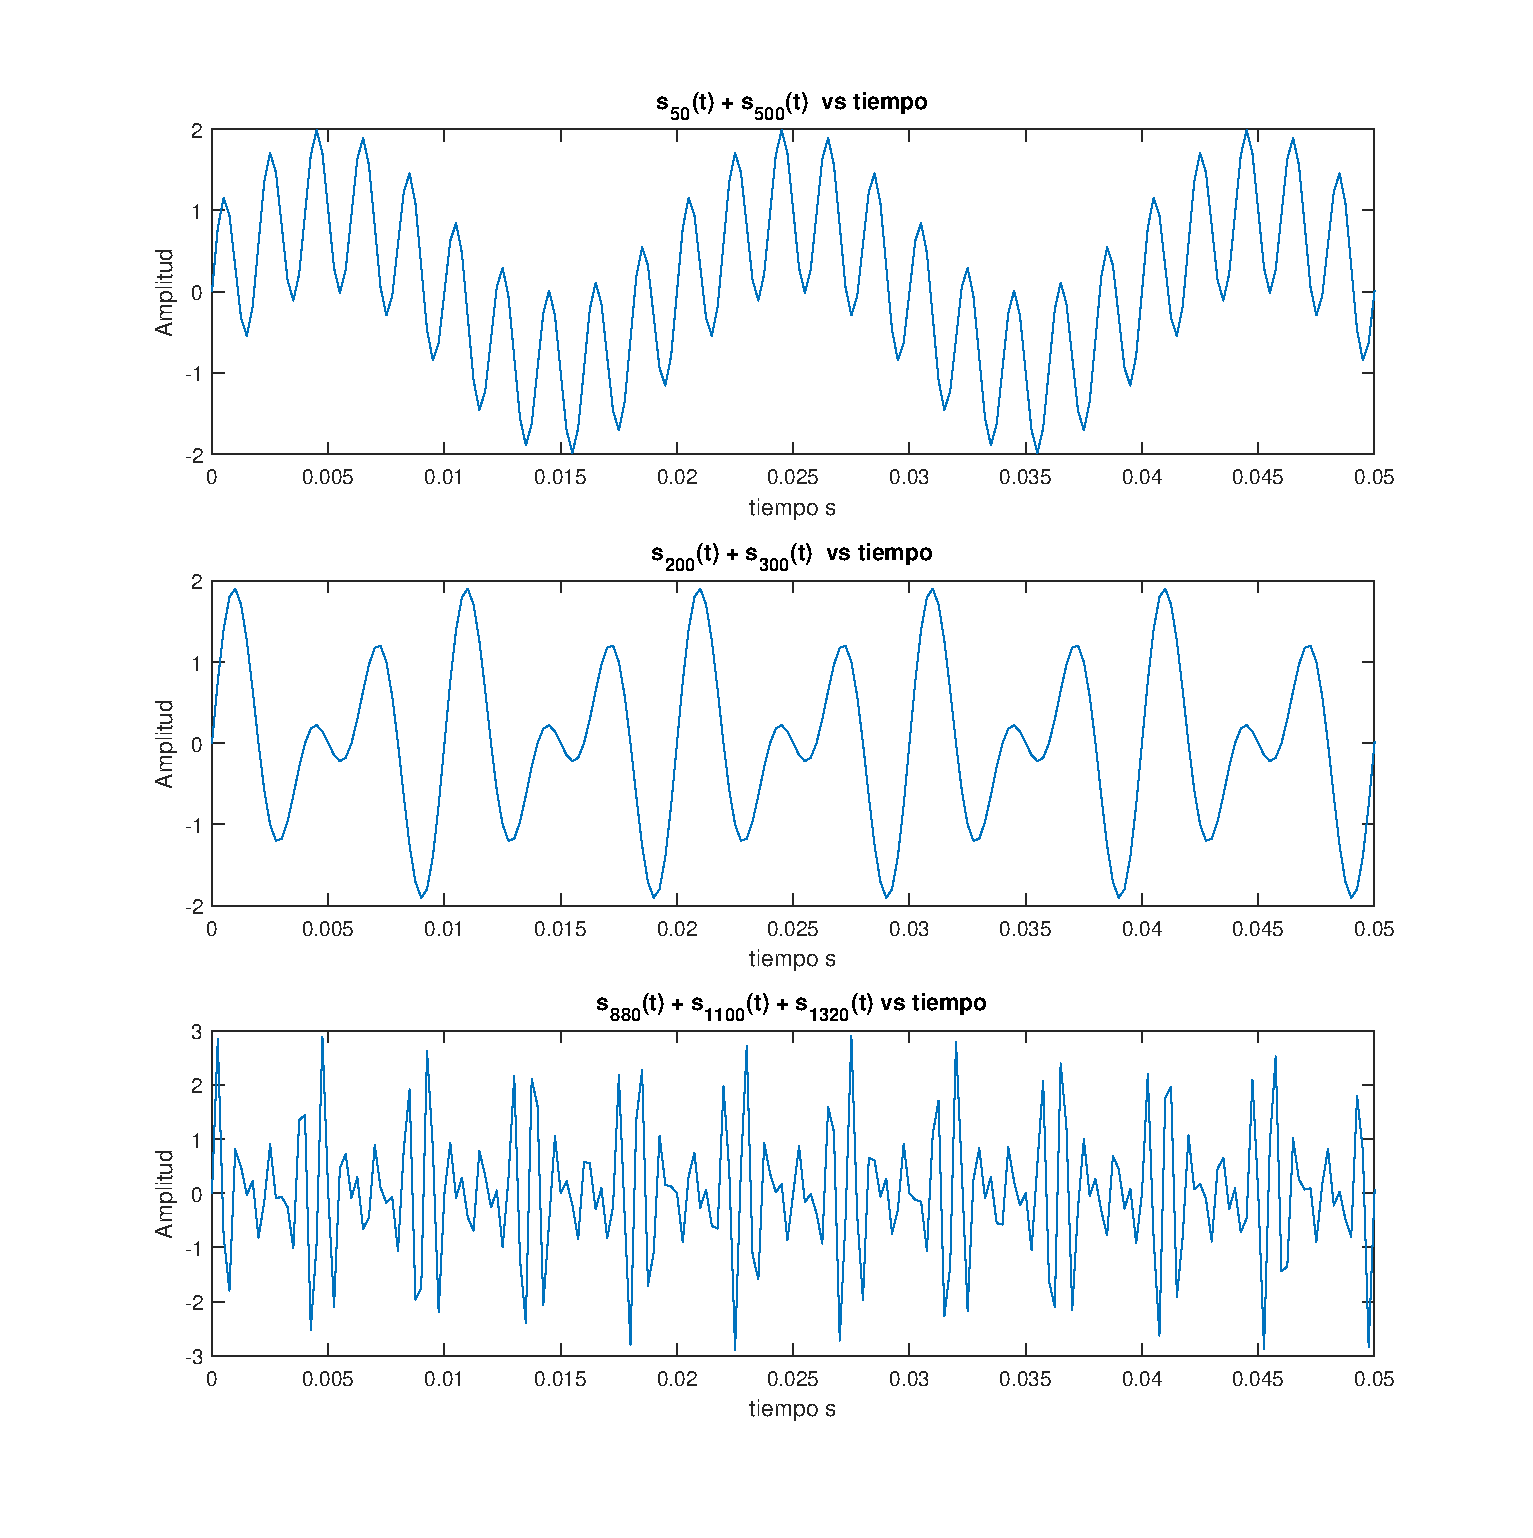
\includegraphics[scale = 0.6]{Imagenes/suma_senos.eps}
        \caption{Gráficas de las señales obtenidas mediante suma de tonos puros.}
        \label{suma_senos}
    \end{figure}
    
    %3
    \item Se desarrolla un  script para sintetizar una aproximación de una señal cuadrada mediante  una componente sinusoidal fundamental sumada a sus armónicos impares desde el 3 al 11, esto considerando fase igual a cero. Siguiendo la expresión siguiente:
    
    
    $$ ss[n] = \sum^6_{k=1} sin(2\pi (2k-1)(f/f_s)n)$$
    
    Obteniendo de esta mandera, la gráfica presente en la figura \ref{sint_fase0}, incrementando cada vez un armónico impar a la serie finita.
    
    \begin{figure}[H]
        \centering
        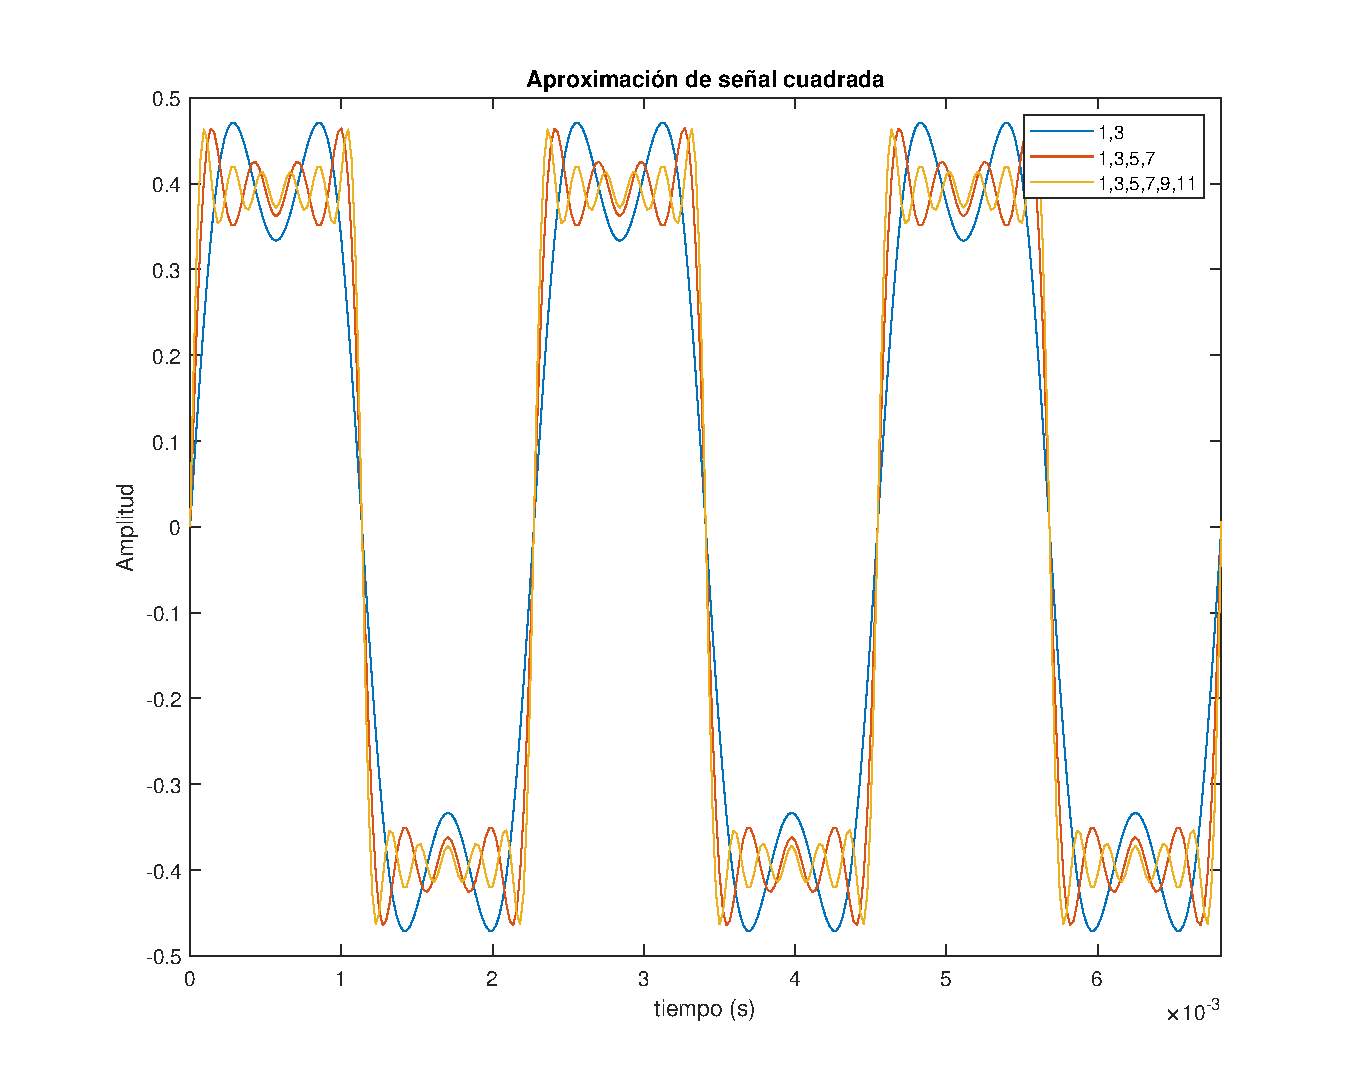
\includegraphics[scale = 0.5]{Imagenes/aproximacion_sennal_cuadrada.eps}
        \caption{Aproximación sintetizada con sinusoidal fundamental y armónicos impares del 3 a 11}
        \label{sint_fase0}
    \end{figure}
    
Luego se modifica el script para poder añadir una fase aleatoria a la aproximación de la señal, siguiendo la siguiente expresión:
    $$ ss[n] = \sum^6_{k=1} sin(2\pi (2k-1)(f/f_s)n + \phi (k))$$


Los resultados de ambos casos se muestran en la figura \ref{sintetizadas}

\begin{figure}[H]
    \centering
    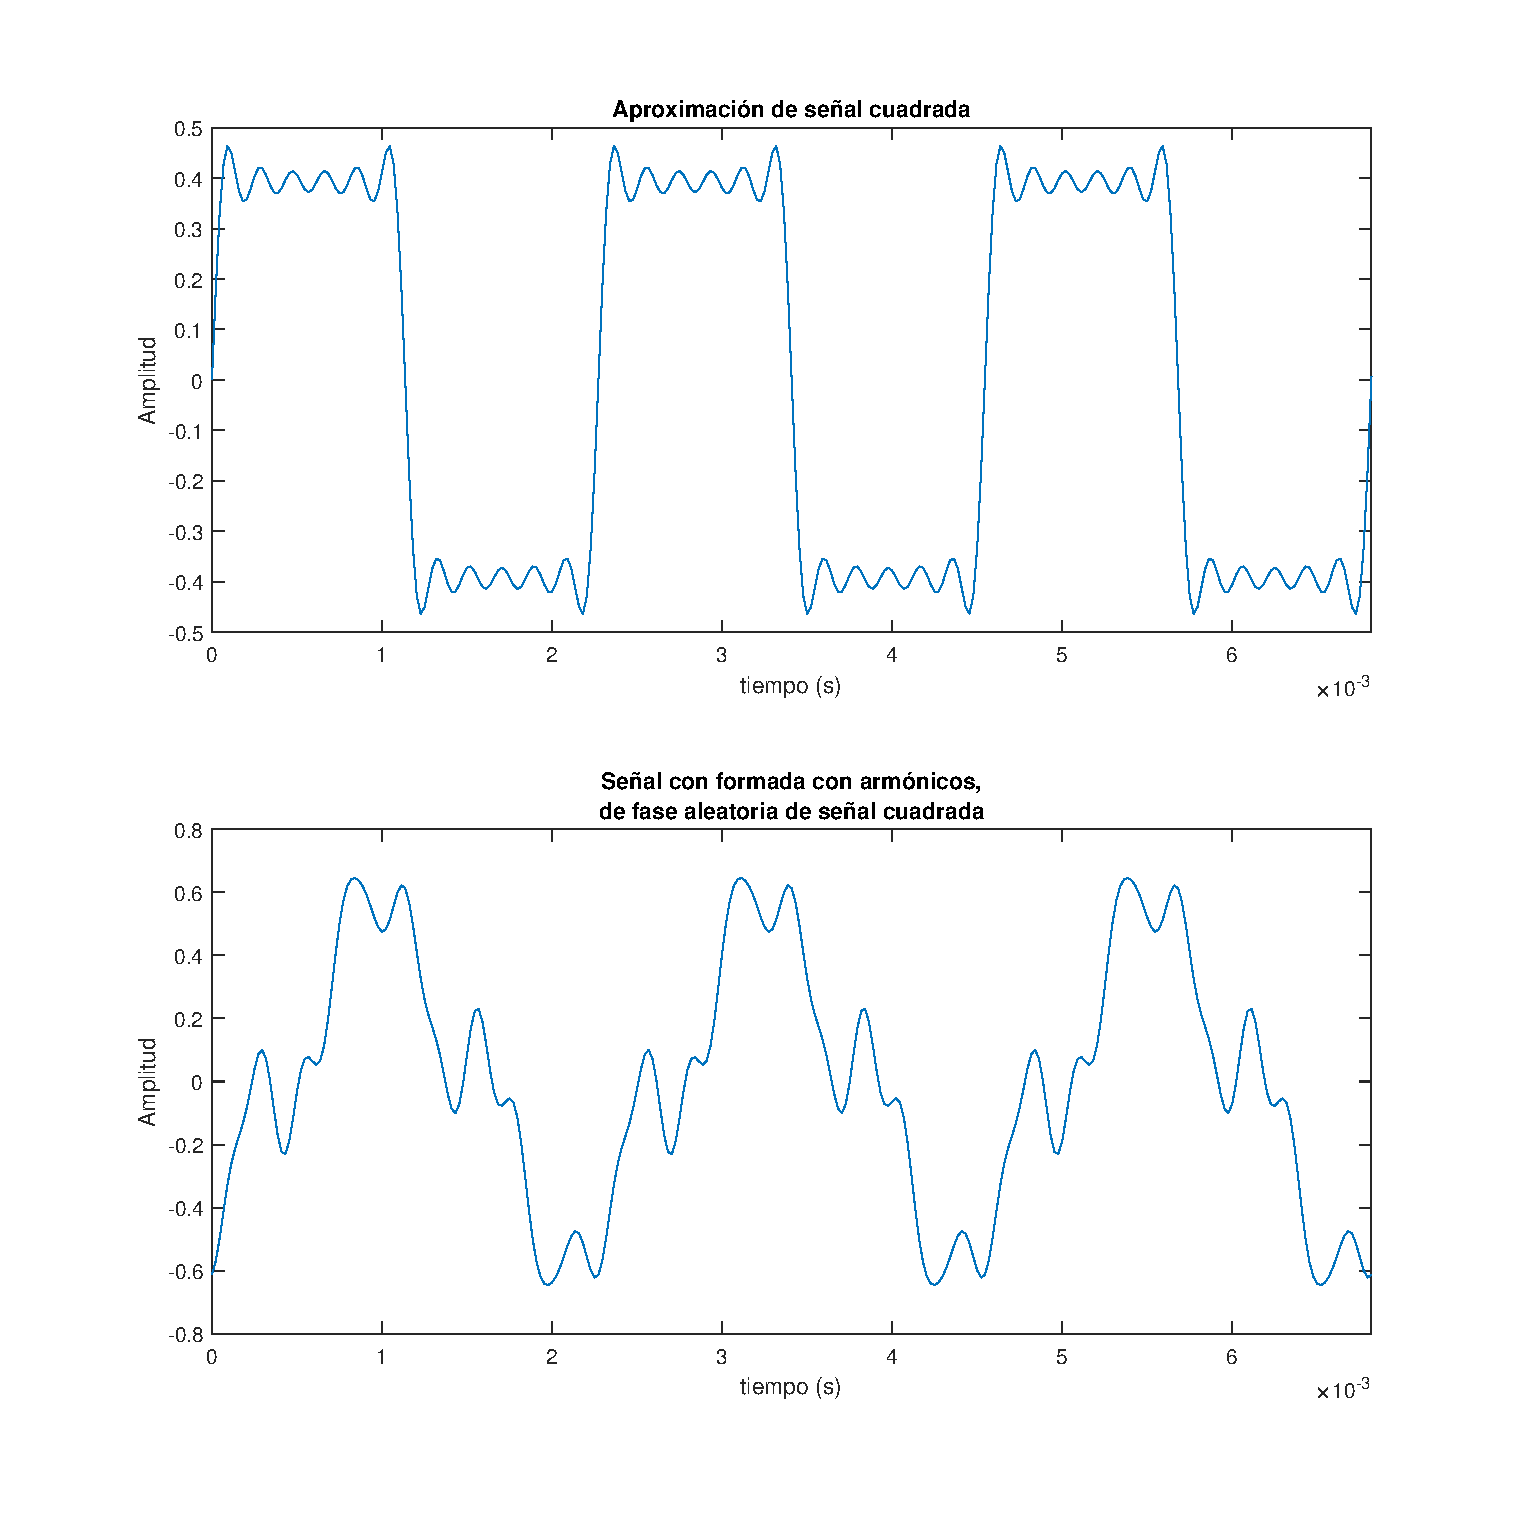
\includegraphics[scale = 0.5]{Imagenes/aprox_cuadrada-armónicos_fase_al.eps}
    \caption{Aproximación sintetizada mediante armónicos tanto con fase cero como con fase aleatoria.}
    \label{sintetizadas}
\end{figure}
    
    
    Para ambas situaciones se utilizó una frecuencia de muestreo de $44~kHz$ para asegurar que se cumpla el criterio de Nyquist para todas las frecuencias presentes en estos experimentos. 
    \newline
    Como se puede apreciar en la figura \ref{sintetizadas} el cambio de fase de las componentes provoca un notorio cambio en la forma de onda de la señal resultante, dejando de acercarse a lo que es una señal cuadrada. Sin embargo,  la frecuencia de ambas señales resultantes (o tono, hablando sobre lo audible) se conserva. 
    En cuanto a la percepción, como ya se mencionó el tono escuchado es el mismo pero el timbre del sonido es ligeramente distinto cuando las formas de ondas obtenidas en fase cero y fase aleatoria son similares, pero en otros casos la forma de onda de la señal generada con fase aleatoria difiere significativamente respecto a la que tiene fase cero, en estas ocasiones el timbre era notablemente distinto entre ambos sonidos.
    
    
    
    
    %4
    \item Se generan señales aleatorias de distribución uniforme en el intervalo $[-1; 1]$ utilizando distintas frecuencias de muestro (2, 10 y 44 kHz), las cuales son usadas como ruido aditivo a la señal discreta obtenida a partir del muestreo de la señal original $\sin(2\pi 500 t)$. Los gráficos de las señales se muestran en la figura \ref{fig:p4}.
    
    \begin{figure}[H]
        \centering
        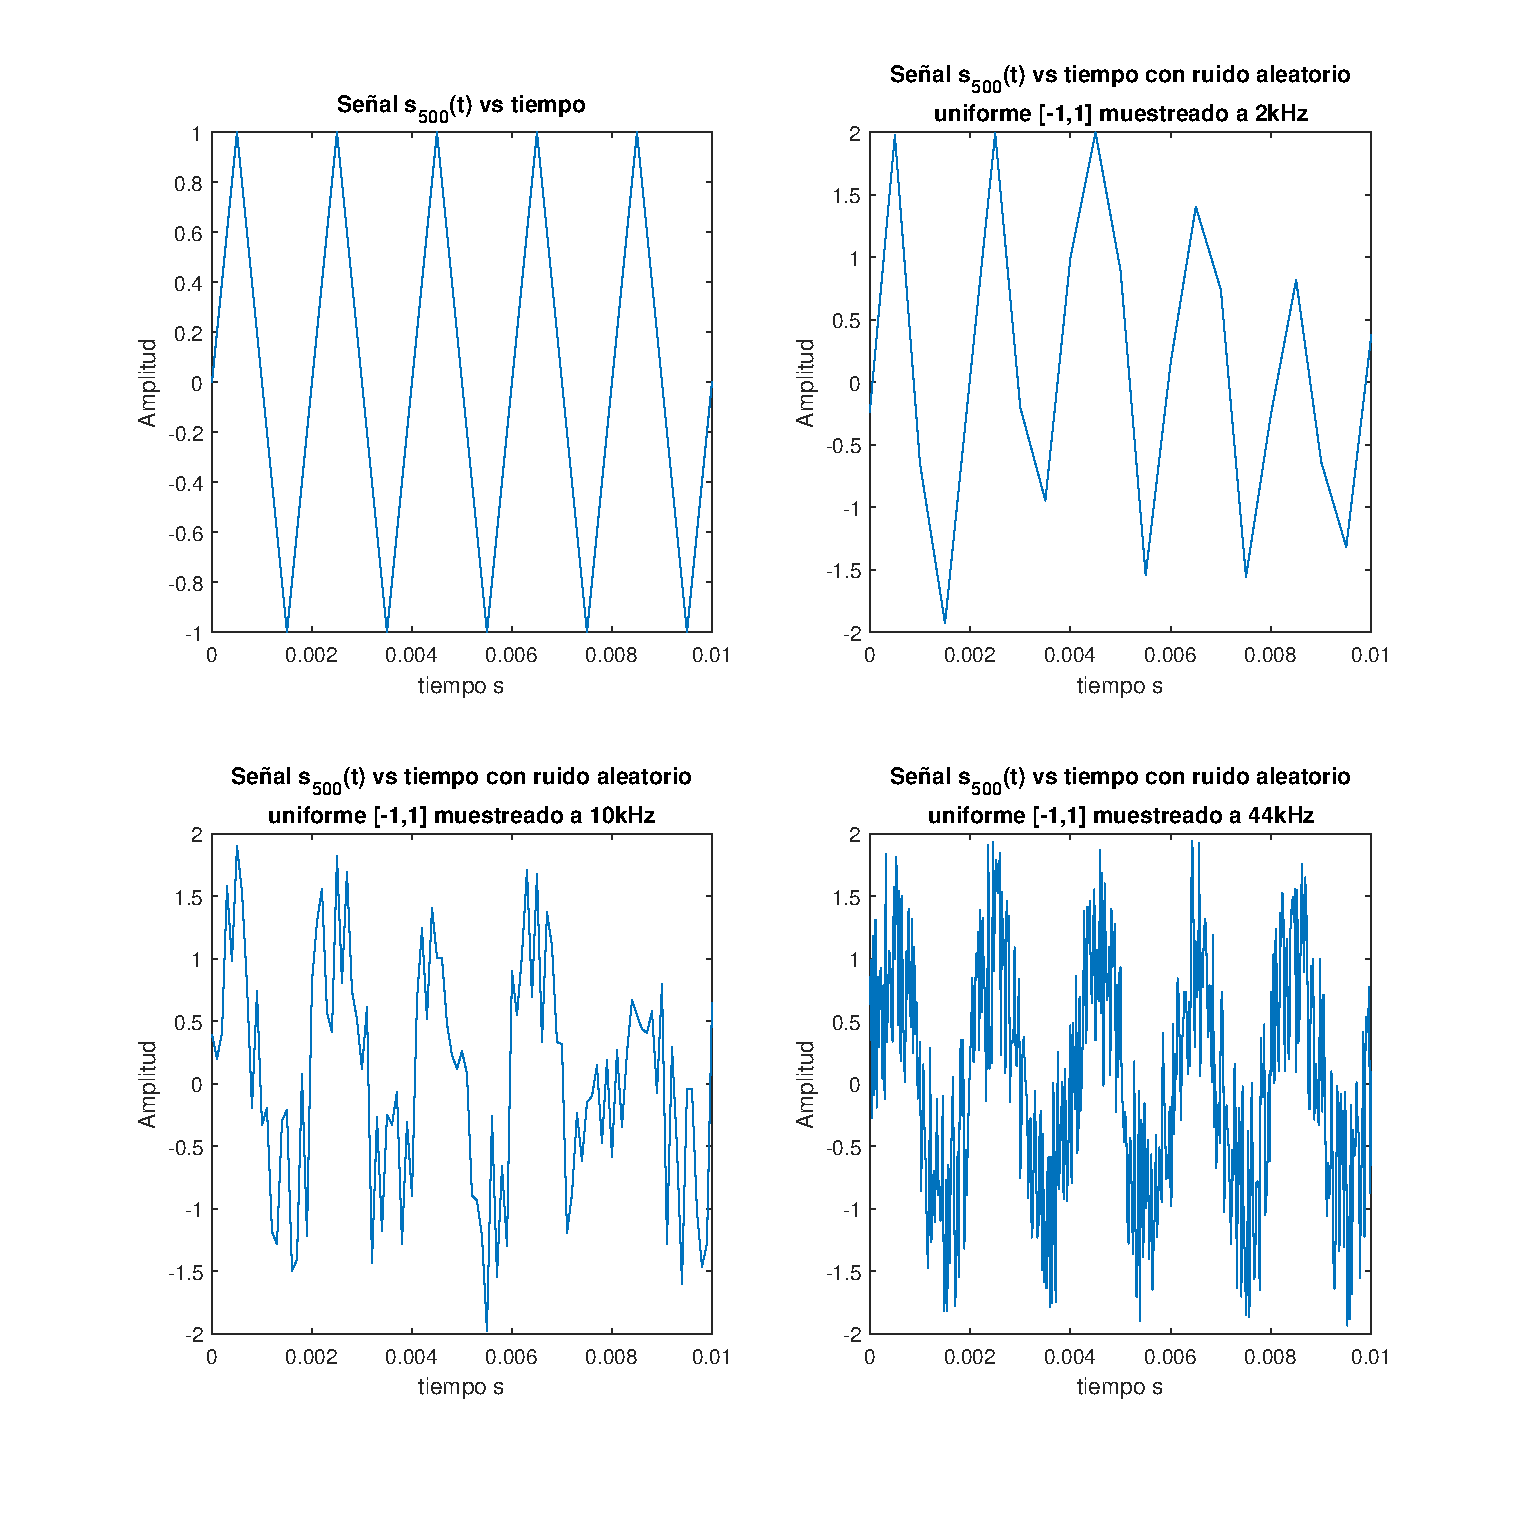
\includegraphics[width = .6\linewidth ]{Imagenes/p4.eps}
        \caption{Primeros 10 ms de señal sinusoidal original y señal generada con amplitud aleatoria.}
        \label{fig:p4}
    \end{figure}
    
    En la figura \ref{fig:p4} se aprecia que a medida que la frecuencia de muestreo aumenta el ruido se hace más evidente. Lo anterior se le atribuye al doblaje en frecuencias ya que a medida que la frecuencia de muestreo aumenta se logra distinguir ruido de alta frecuencia. Se concluye que muestrear a sobretasa (en términos de Nyquist) para una señal que presenta ruido aditivo puede ser contraproducente.
    
    %5
    \item Se pide modificar la señal sinusoidal original de 500 Hz de modo que la amplitud varíe aleatoriamente entre $[0.5;1]$. Se utiliza una distribución uniforme en este intervalo.
    
    El gráfico de los primeros 10 ms de la nueva señal y original se muestra en \ref{fig:p5}.
    
    \begin{figure}[H]
        \centering
        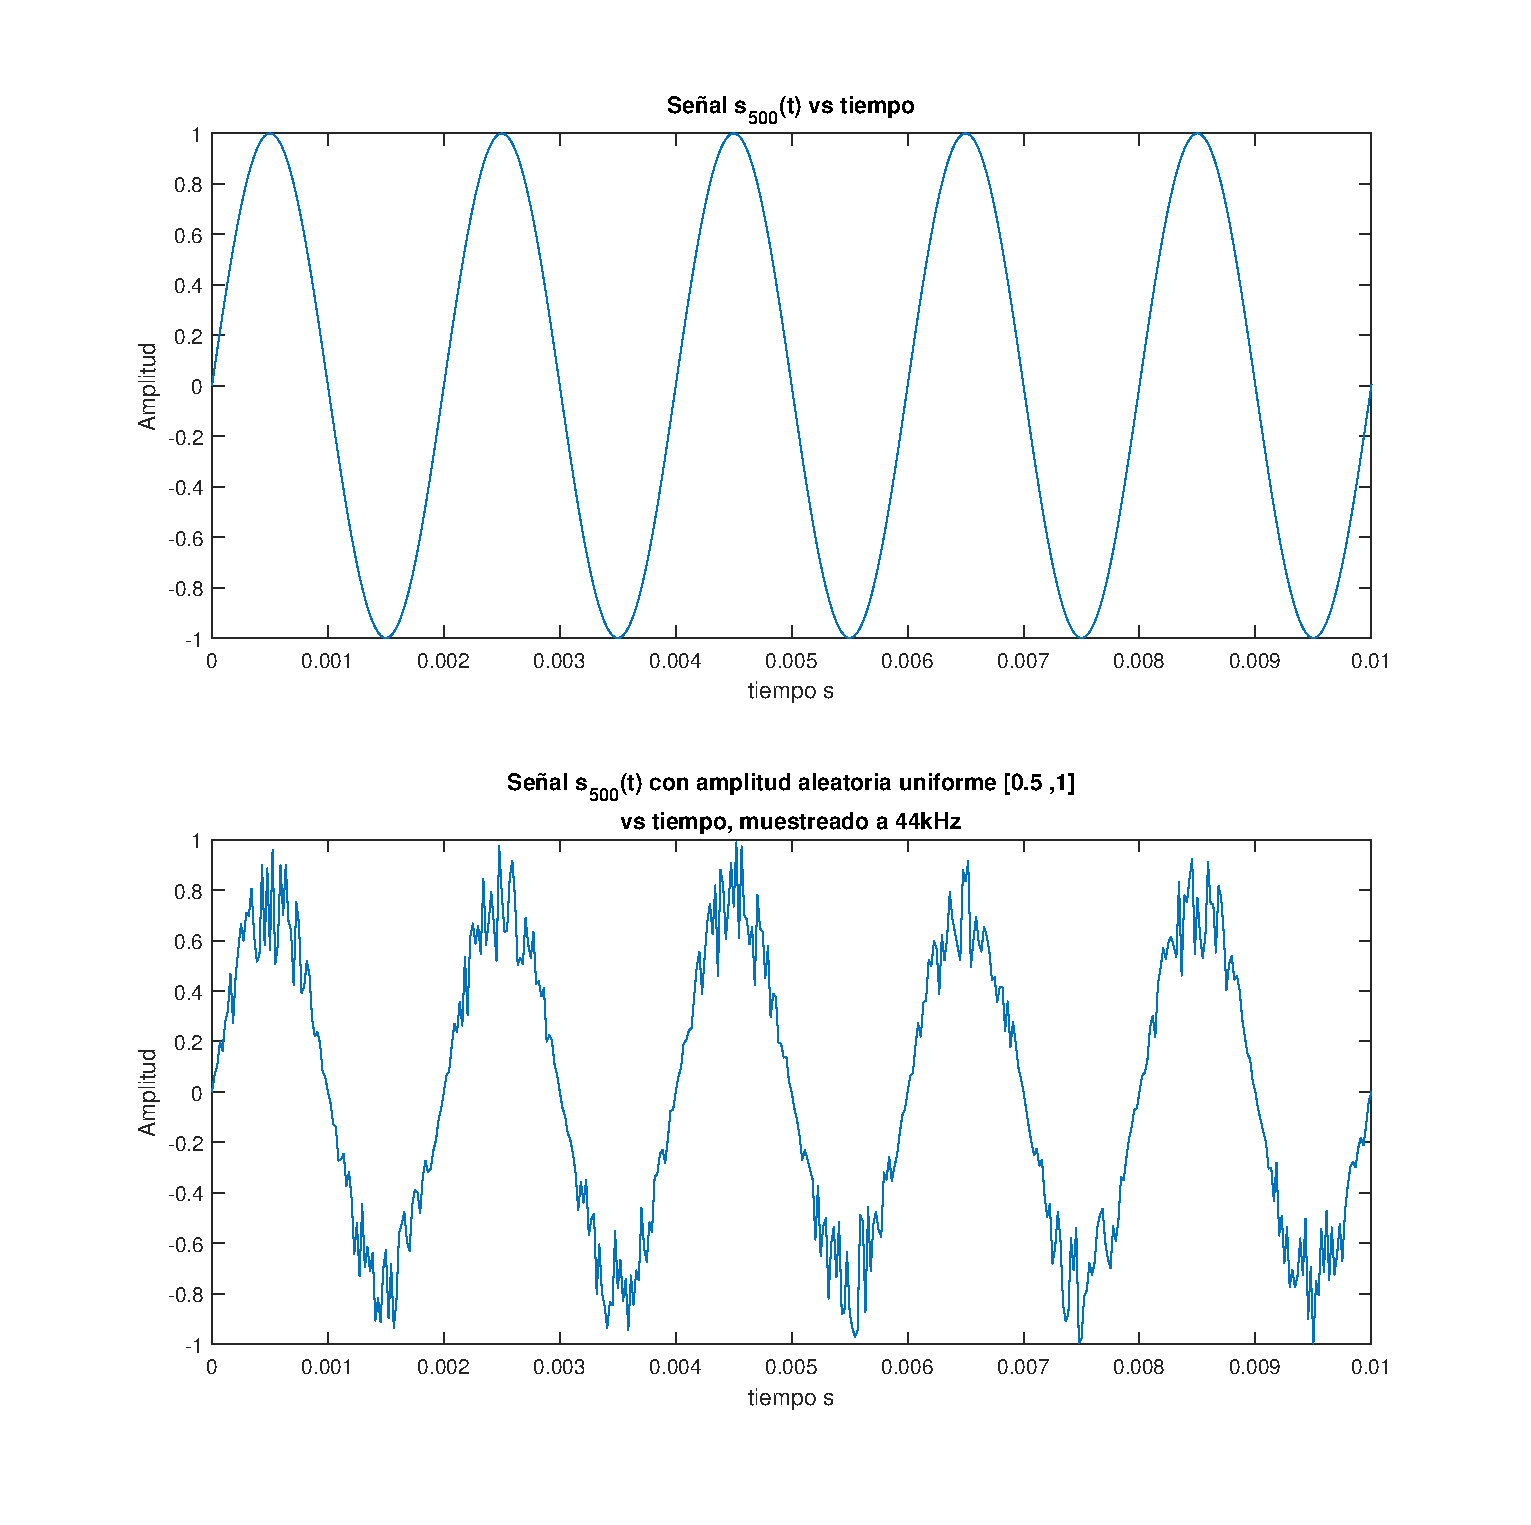
\includegraphics[width = .6\linewidth ]{Imagenes/p5.eps}
        \caption{Primeros 10 ms de señal sinusoidal original y señal generada con amplitud aleatoria.}
        \label{fig:p5}
    \end{figure}
    
    %6
    \item Se pide modificar la señal sinusoidal original de 500 Hz de modo que su fase varíe aleatoriamente entre $[\pi/2;\pi/2]$. Se utiliza una distribución uniforme en este intervalo.
    
    El gráfico de los primeros 10 ms de la nueva señal y original se muestra en \ref{fig:p6}.
    
    \begin{figure}[H]
        \centering
        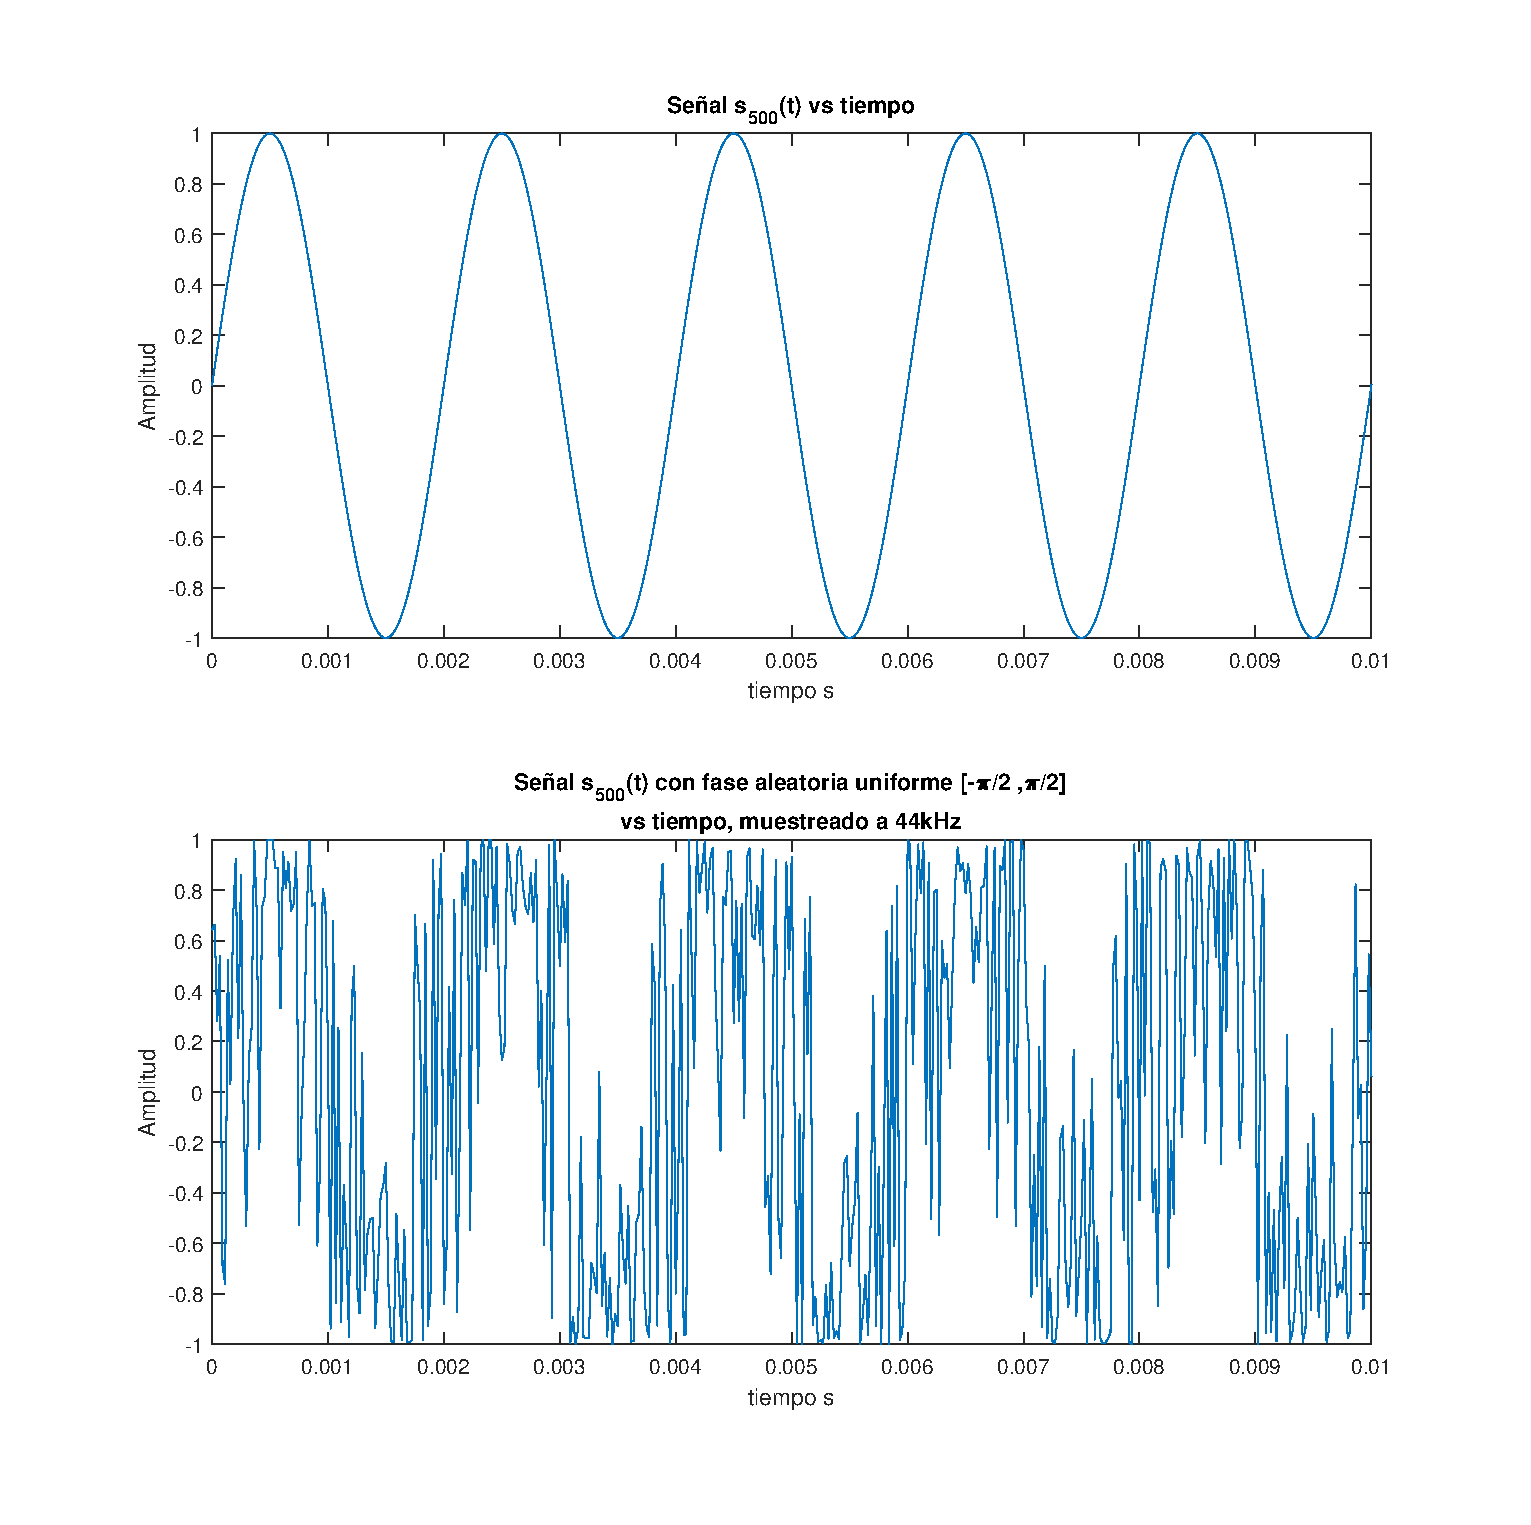
\includegraphics[width = .6\linewidth ]{Imagenes/p6.eps}
        \caption{Primeros 10 ms de señal sinusoidal original y señal generada con fase aleatoria.}
        \label{fig:p6}
    \end{figure} 
    
    %7
    \item Con respecto a los tipos de ruido con los que se experimentó en los puntos anteriores, se observa que:
    \begin{itemize}
        \item El ruido aditivo afecta a los valores puntuales de la señal, sin emargo, visualmente la frecuencia de la señal es distinguible. Esta propiedad es interesante al pensar en modulación FM en un canal. 
        
        
        \item El ruido en amplitud resulta visualmente evidente cuando el valor de la señal sinusoidal es alto. Comparativamente es el menos dañino para la señal original. 
        
        \item La fase aleatoria es, comparativamente, el tipo de ruido que genera mayor deformación de la señal original.
    \end{itemize}
    
    Con respecto a la percepción auditiva de las señales generadas se puede comentar que:
    
    \begin{itemize}
        \item Para los audios generados con ruido aditivo, a medida que se aumenta la frecuencia de muestreo el ruido se vuelve más ''rico'' en frecuencias. Sintiendose grave para 2 kHz y molestamente agudo a 44 kHz.
        
        \item La amplitud aleatoria genera el ruido mas suave sobre la señal original, como se esperaba del análisis visual.
        
        \item La fase aleatoria genera un ruido perceptualmente similar la aditiva, sin embargo, la razón perceptual entre el ruido y la señal original es claramente mayor que en el caso aditivo. Probablemente la SNR en esta señal es menor.
    \end{itemize}
    
    
    
    
    
    
    
    
\end{enumerate}